\documentclass{beamer}
\usetheme{Berkeley}

\usepackage{default}
\usepackage{xspace}
\usepackage{algorithm}
\usepackage[noend]{algpseudocode}
\usepackage{listings}
\usepackage{tikz}
\usepackage{tkz-graph}
\usetikzlibrary{arrows,%
	petri,%
	topaths,
	calc}%

\newcommand{\TODO}[1]{\noindent\textcolor{green}{\textbf{TODO:} #1}}

\newcommand{\pathfinder}{\textsc{Pathfinder}\xspace}
\newcommand{\findEdgeCandidates}{FindEdgeCandidates\xspace}
\newcommand{\refineEdgeCandidates}{RefineEdgeCandidates\xspace}
\newcommand{\getAssociatedTrajectories}{GetAssociatedTrajectories\xspace}
\newcommand{\chrep}{CH-representation\xspace}

\title[Pathfinder] % (optional, only for long titles)
{PATHFINDER}
\subtitle{Storage and Indexing of Massive Trajectory Sets}
\author[Funke, Nusser, Rupp, Storandt] % (optional, for multiple authors)
{S.~Funke\inst{1} \and A.~Nusser\inst{2} \and T.~Rupp\inst{3} \and S.~Storandt\inst{4}}
\institute[Universities] % (optional)
{
	\inst{1}%
	University of Stuttgart
	\and
	\inst{2}%
	Max Planck Institute for Informatics
	\and
	\inst{3}%
	University of Stuttgart
	\and
	\inst{4}%
	University of Konstanz
}
\date[SSTD 2019] % (optional)
{SSTD, 2019}
\subject{Computer Science}


\begin{document}
\frame{\titlepage}

\frame{\tableofcontents[
		currentsection,
		currentsubsection,
		subsectionstyle=show/shaded/hide
	]}

\section{Problem Description}
\begin{frame}
	\frametitle{Problem Description}
	\begin{itemize}
		\item<1-> road network graph $G(V,E,c)$
		\item<2-> trajectory data is provided as a collection $\mathcal{T}$
		\item<3-> $t\in \mathcal{T}$ is a sequence of nodes $\pi=v_0 v_1 \dots v_k$ in  $G$ annotated with timestamps $\tau_0, \tau_1, \dots, \tau_k$.
		\item<4-> \emph{window}-query of the form $[x_l, x_u]\times[y_l, y_u]\times[\tau_l, \tau_u]$
		\item<5-> goal: Return all intersecting trajectories
	\end{itemize}
\end{frame}

\section{Preliminaries}
\begin{frame}
	\frametitle{Contraction Hierarchy}
	\begin{itemize}
		\item<1-> CH is a augmentation of a graph $G(V,E,c)$ with \emph{shortcuts} and \emph{node levels}.
		\item<2-> \emph{node contraction}: removes a node $v$ and all of its adjacent edges from the graph
		\item<3-> To maintain shortest path distances in the graph: Create shortcut $s = (u, w)$ between two adjacent nodes $u,w$ of $v$ if the only shortest path from $u$ to $w$ is the path $uvw$. $c(s) = c(uv) + c(vw)$.
		\item<4-> Construct CH by successively contracting all nodes
		\item<5-> final CH data structure is defined as $G(V, E^+, c, l)$ where $E^+$ is the union of $E$ and all shortcuts
	\end{itemize}
\end{frame}

\begin{frame}
	\frametitle{Shortcut Representation}
	\framesubtitle{Compression}
	\begin{figure}
		\TODO{step by step picture}
		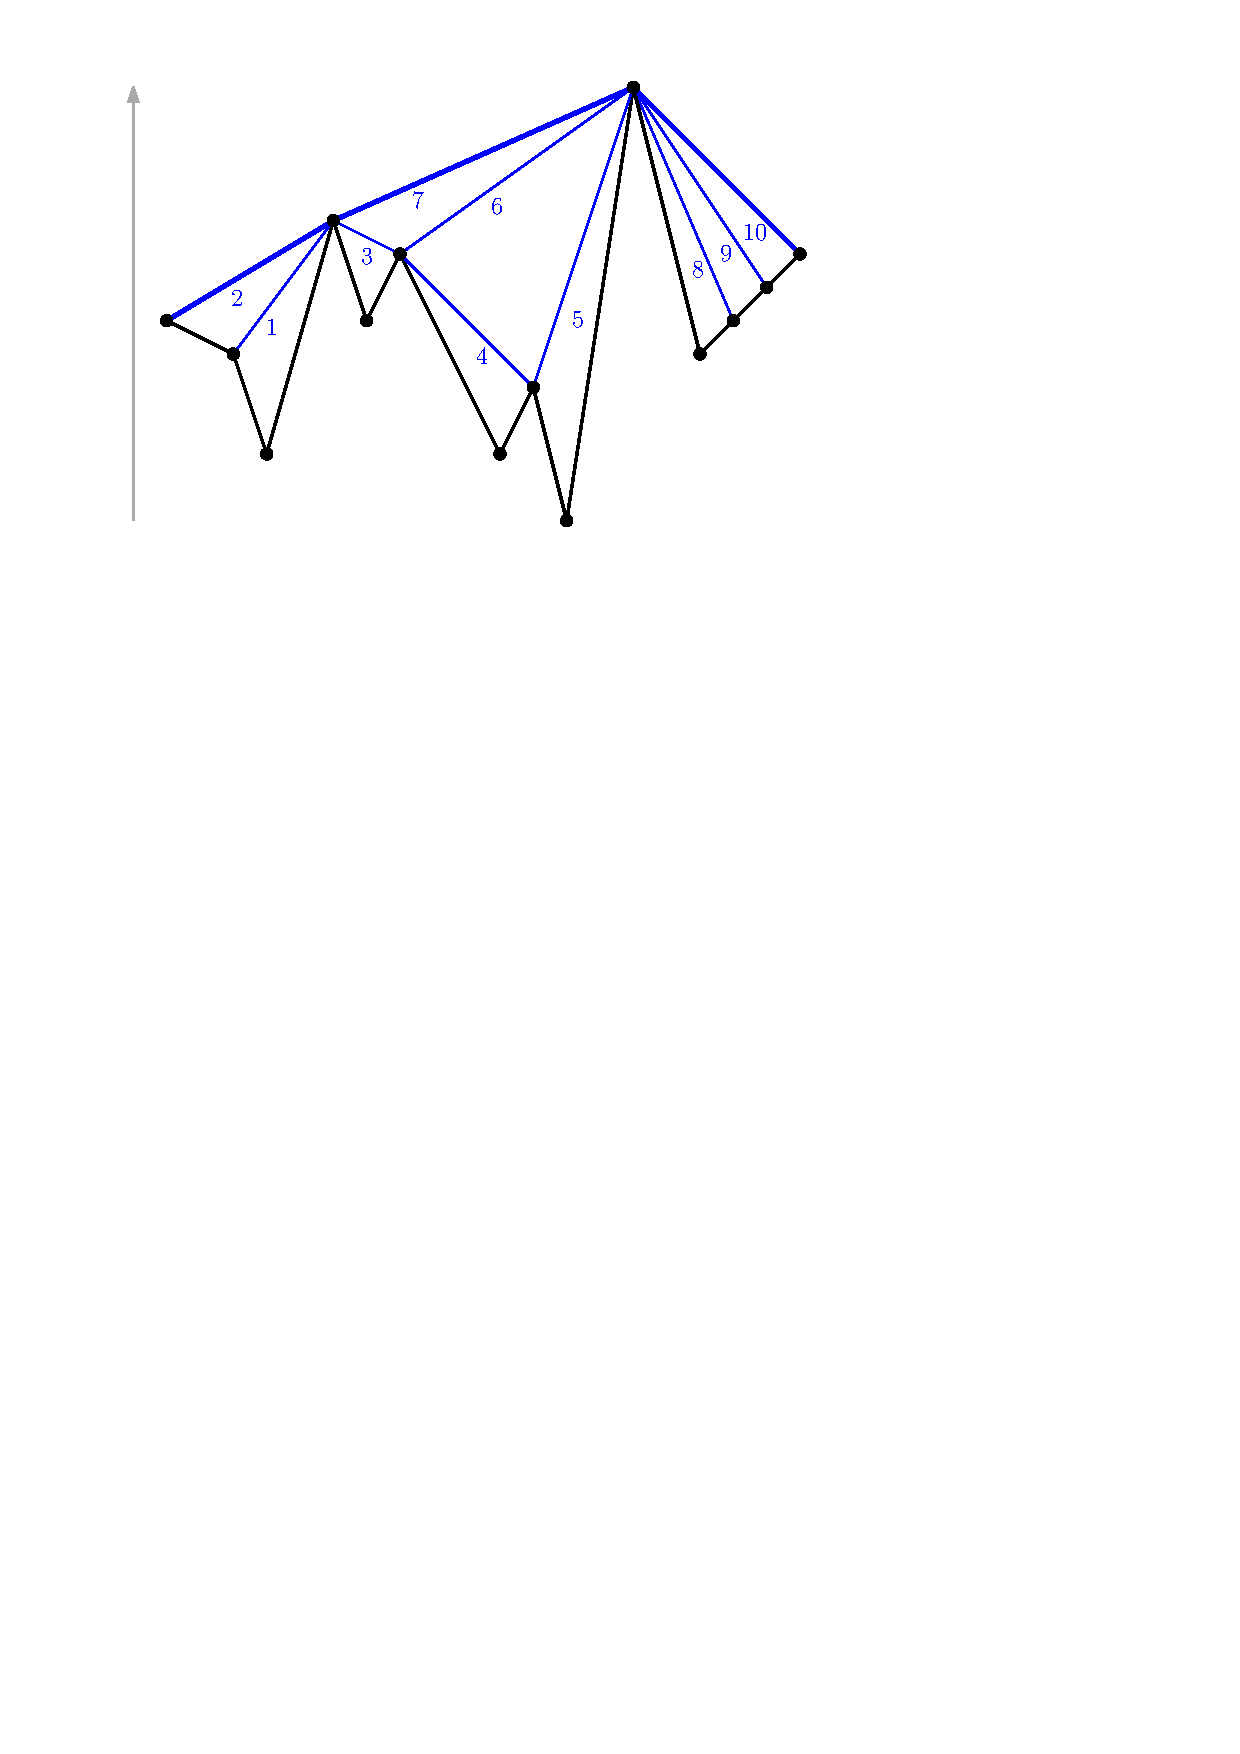
\includegraphics[width=.76\columnwidth]{images/toch}
		\caption{Original path (black) and derivation of its \chrep (bold blue) via repeated shortcut substitution. $y$-coordinate corresponds to CH level.}
	\end{figure}
\end{frame}

\begin{frame}
	\frametitle{CH as RTree}
\end{frame}

\section{Algorithm}

\begin{frame}
	\frametitle{Algorithm Overview}
	Inverted Index: Associate a trajectory with all edges of its \chrep in $E^+$.
	\begin{algorithm}[H]
		{\small
			\caption{Spatial \pathfinder Algorithm}
			\begin{algorithmic}[1]
				\Procedure{PathfinderQuery}{$Q$} \pause
				\State $E_O \gets \Call{\findEdgeCandidates}{Q}$ \label{line:edge_revrieval} \pause
				\State $E_r \gets \Call{\refineEdgeCandidates}{Q, E_O}$ \pause
				\State \Return $\Call{\getAssociatedTrajectories}{E_r}$
				\EndProcedure
			\end{algorithmic}
			\label{alg:spatial_pathfinder}
		}
	\end{algorithm}
\end{frame}

\subsection{\findEdgeCandidates}
\begin{frame}
	\frametitle{\findEdgeCandidates}
	\framesubtitle{Path box}
	\emph{Path box} $PB(e)$: Bounding box for the path that an edge $e$ represents.
	\TODO{illustration}
\end{frame}

\begin{frame}
	\frametitle{\findEdgeCandidates}
	\framesubtitle{Downgraph box}
	\TODO{mach grünes kleiner}
	\emph{Downgraph box} $DB(v)$: Bounding box of all nodes that are reachable from a node $v$ on a down-path (only visiting nodes of decreasing CH-level)
	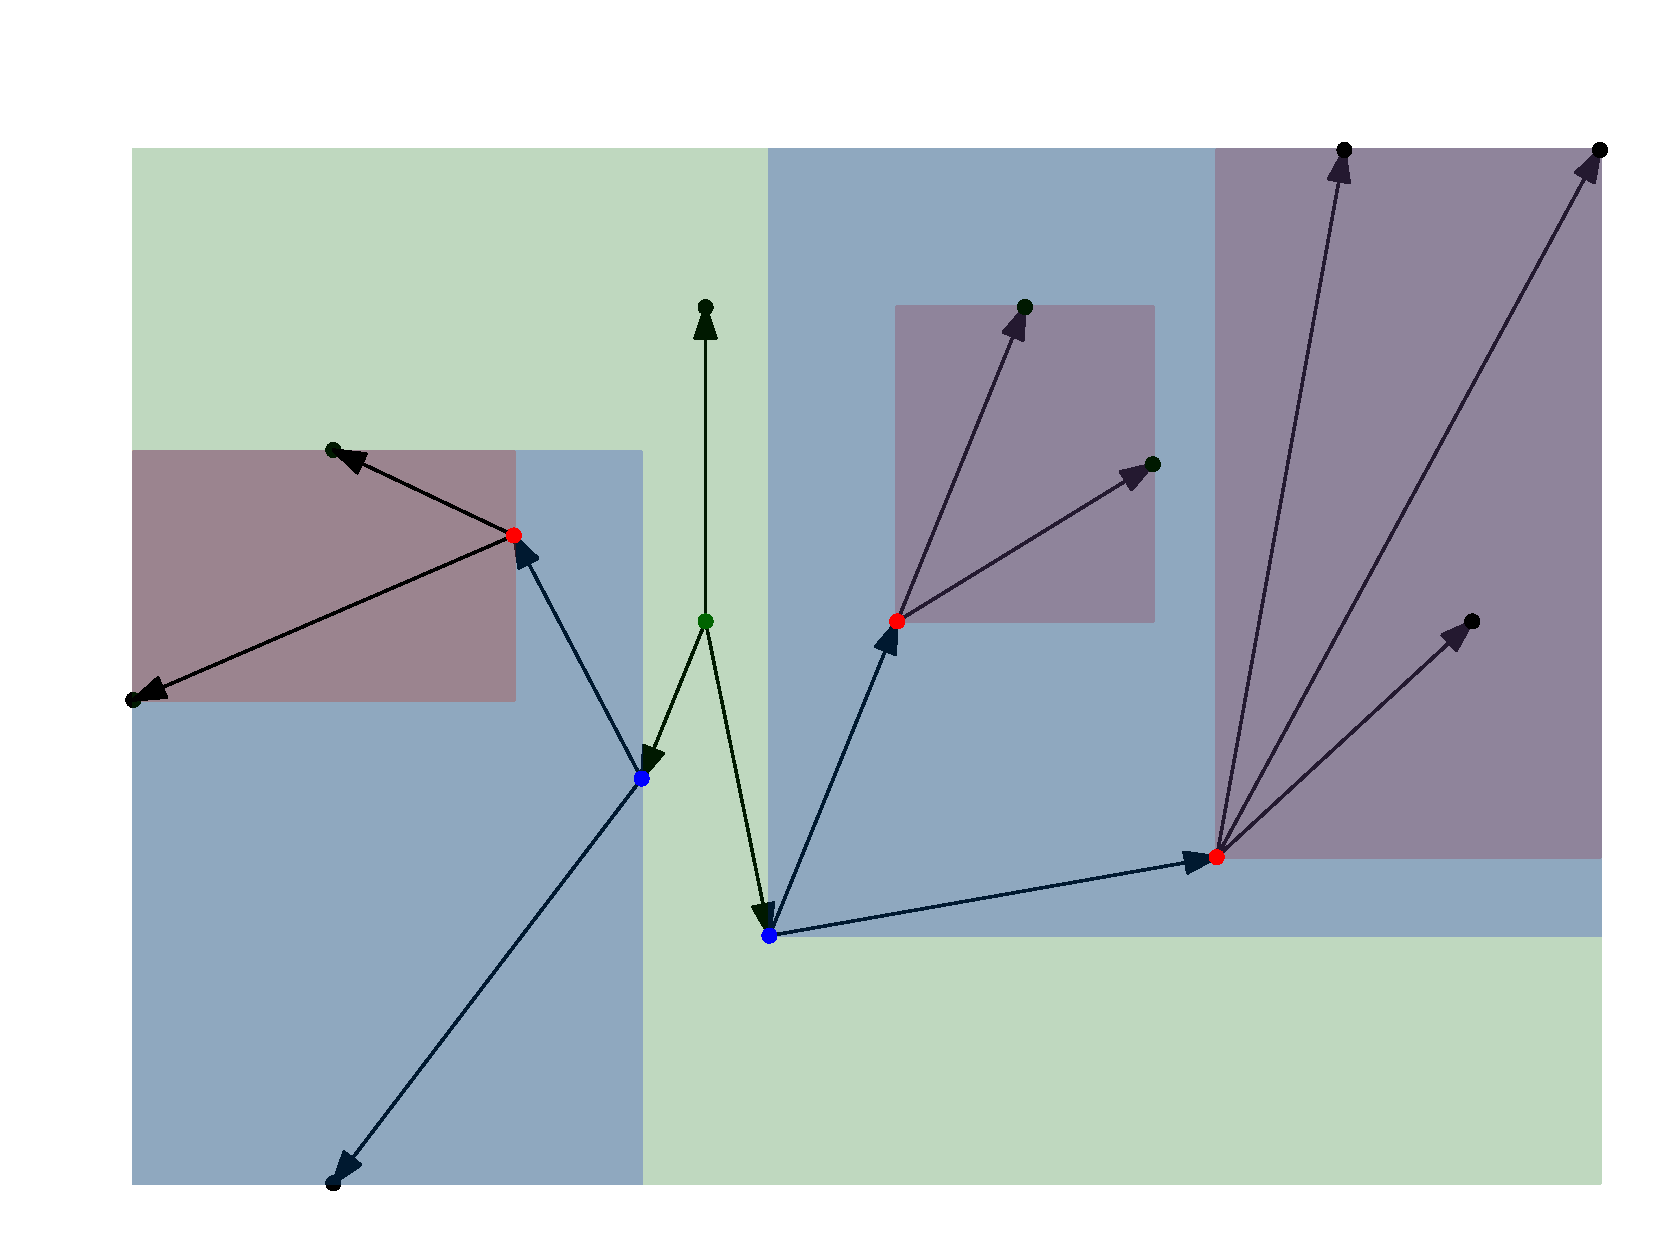
\includegraphics[width=.76\columnwidth]{images/downgraphBox}
\end{frame}

\begin{frame}
	\frametitle{\findEdgeCandidates}
	\TODO{mach grünes kleiner}
	\begin{algorithm}[H]
		{\small
			\caption{The algorithm to find edge candidates given a query rectangle $Q$.}
			\begin{algorithmic}[1]
				\Procedure{\findEdgeCandidates}{$Q$}
				\State $V_T \gets \Call{FetchTopNodes}{Q}$
				\State $E_O \gets \emptyset$
				\For {$v \in V_T$}
				\State $E_O \gets E_O \cup \Call{FindCandidatesForNode}{v, Q}$
				\EndFor
				\State \Return $E_O$
				\vspace{0.2cm}
				\EndProcedure
			\end{algorithmic}
		}
	\end{algorithm}
\end{frame}

\begin{frame}
	\frametitle{\findEdgeCandidates}
	\TODO{mach grünes kleiner}
	\begin{algorithm}[H]
		{\small
			\caption{The algorithm to find edge candidates given a query rectangle $Q$.}
			\begin{algorithmic}[1]
				\Procedure{FindCandidatesForNode}{$v, Q$}
				\State $C \gets \emptyset$
				\For {$e \in \text{down edges of $v$}$}
				\If {$PB(e) \cap Q \neq \emptyset$}
				\State $C \gets C \cup \{e\}$
				\EndIf
				\State $v_l \gets \text{lower node of $e$}$
				\If {$DB(v_l) \cap Q \neq \emptyset$}
				\State $C \gets C \cup \Call{FindCandidatesForNode}{v_l, Q}$
				\EndIf
				\EndFor
				\State \Return $C$
				\EndProcedure
			\end{algorithmic}
		}
	\end{algorithm}
	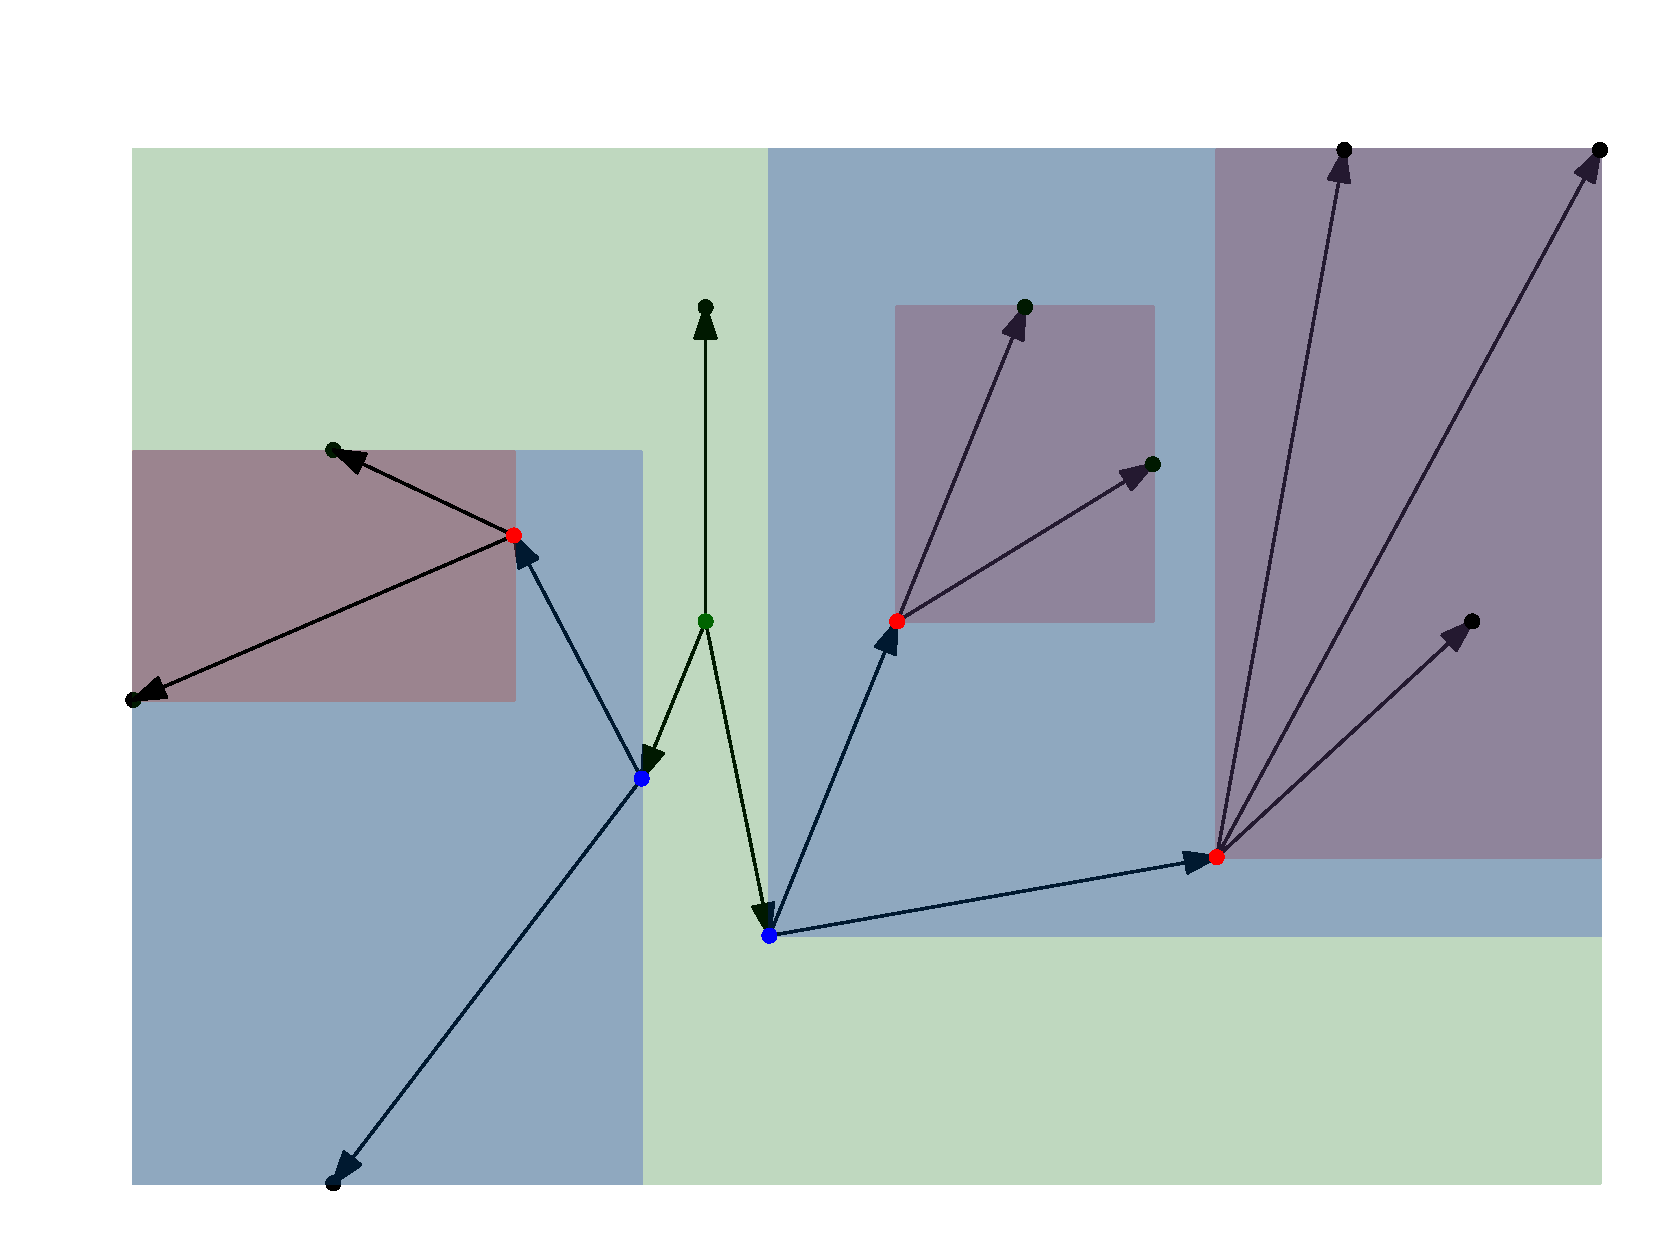
\includegraphics[width=.76\columnwidth]{images/downgraphBox}
\end{frame}

\subsection{\refineEdgeCandidates}
\begin{frame}
	\frametitle{\refineEdgeCandidates}
	Problem: Some of the candidates my be false positives. \pause

	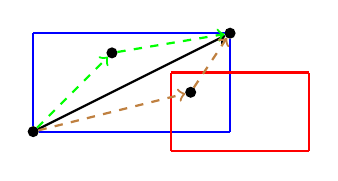
\begin{tikzpicture}

		\SetGraphUnit{1}

		\GraphInit[vstyle=Classic]
		\tikzset{VertexStyle/.style =
				{shape=circle, fill=black, minimum size = 4pt,inner sep=0pt}
		}

		%edge
		\tikzstyle{EdgeStyle}=[->, color=black]
		\SetVertexNoLabel
		\Vertex[x=-0.5,y=2]{source}
		\Vertex[x=2,y=3.25]{target}

		\Edge(source)(target) {e}


		%edgeBox

		\tikzset{VertexStyle/.style =
				{shape=circle, fill=black, minimum size = 0pt,inner sep=0pt}
		}
		\SetVertexNoLabel
		\Vertex[x=2,y=2]{6}
		\Vertex[x=-0.5,y=3.25]{8}

		\tikzstyle{EdgeStyle}=[color=blue]
		\Edge(source)(6)
		\Edge(6)(target)
		\Edge(target)(8)
		\Edge(8)(source)


		%queryBox
		\Vertex[x=1.25,y=1.75]{1}
		\Vertex[x=3,y=1.75]{2}
		\Vertex[x=3,y=2.75]{3}
		\Vertex[x=1.25,y=2.75]{4}

		\tikzstyle{EdgeStyle}=[color=red]
		\Edge(1)(2)
		\Edge(2)(3)
		\Edge(3)(4)
		\Edge(4)(1)

		%unpacked
		\tikzset{VertexStyle/.style =
				{shape=circle, fill=black, minimum size = 4pt,inner sep=0pt}
		}

		%possibility1
		\Vertex[x=0.5,y=3, LabelOut=true, Lpos=-90]{9}

		\tikzstyle{EdgeStyle}=[->, color=green, dashed]
		\Edge(source)(9)
		\Edge(9)(target)

		%possibility2
		\Vertex[x=1.5,y=2.5, LabelOut=true, Lpos=180]{10}

		\tikzstyle{EdgeStyle}=[->, color=brown, dashed]
		\Edge(source)(10)
		\Edge(10)(target)
	\end{tikzpicture}
	\pause

	Here the black edge $e$ is a candidate because of $PB(e) \cap Q \neq \emptyset$. \pause

	If $e$ bridges \pause
	\begin{itemize}
		\item intersecting brown path  $\Rightarrow$ true positive \pause
		\item non-intersecting green path $\Rightarrow$ false positive \pause
	\end{itemize} \pause
	$\Rightarrow$ in doubt, $e$ have to be unpacked recursively
\end{frame}

\subsection{\getAssociatedTrajectories}
\begin{frame}
	\frametitle{\getAssociatedTrajectories}
\end{frame}

\section{Extensions}

\subsection{Time frame quries}
\begin{frame}
	\frametitle{TimeFrameQueries}
\end{frame}

\subsection{Parallelization}
\begin{frame}
	\frametitle{Parallelization}
\end{frame}

\subsection{On disk storage}
\begin{frame}
	\frametitle{OnDisk (SSTD)}
\end{frame}

\section{Experiments}

\begin{frame}
	\frametitle{Experiments}
	\framesubtitle{Hardware}
\end{frame}

\begin{frame}
	\frametitle{Experiments}
	\framesubtitle{Data}
\end{frame}

\begin{frame}
	\frametitle{Experiments}
	\framesubtitle{Evaluations compression}
\end{frame}

\begin{frame}
	\frametitle{Experiments}
	\framesubtitle{Evaluations retrieval}
\end{frame}
% etc
\end{document}
